\chapter{Technologies and Architecture}
\label{cha:456}
This chapter describes the Python modules used to build and run the Dashboards, and how they are structured.\\
The vital signs dashboards have been constructed as a dynamic website that allows user interaction.\\
Let us now describe the role of each Python module.

\section{Plotly}
\label{sec:plotly}
Plotly is a Python graphing library that provides a wide variety of charts for visualising data.
Since we get to plot different data, we need different charts to provide the best suited graph for each data we want to visualize. Each of them is interactive. \\
We remind that the goal of the project is to make the user understand what is going on with Wikipedia health metrics.\\
The power of Plotly is that it allows the graphs to change which data column to show, so the user has the possibility to see exactly the data he or she is interested in: from the time period to the value type.
To create the graphs we use two different sub-modules of Plotly:
\begin{itemize}
    \item \textbf{Graph objects \cite{go}:} The figures created, manipulated and rendered by this plotly Python library are represented by tree-like data structures which are automatically serialized to JSON. These trees are composed of named nodes called ``attributes''. The \verb#plotly.graph# objects module, imported as \verb#go#, contains an automatically-generated hierarchy of Python classes which represent non-leaf nodes in this figure schema. The term "graph objects" refers to instances of these classes.
    \item \textbf{Plotly express \cite{px}:} The Plotly express module, imported as \verb#px#, contains functions that can create entire figures at once. It is a built-in part of the Plotly library, and is the starting point for creating most common figures. Every Plotly Express function uses graph objects internally and returns a Plotly \verb#go.Figure# instance.
    The module \verb#px# was preferred due to its simplicity and more expressive syntax. 
\end{itemize}
In the visual dashboards, we find four different type of graphs:
\begin{figure}[!ht]
  \centering
  \setlocalecaption{english}{figure}{Figure}
  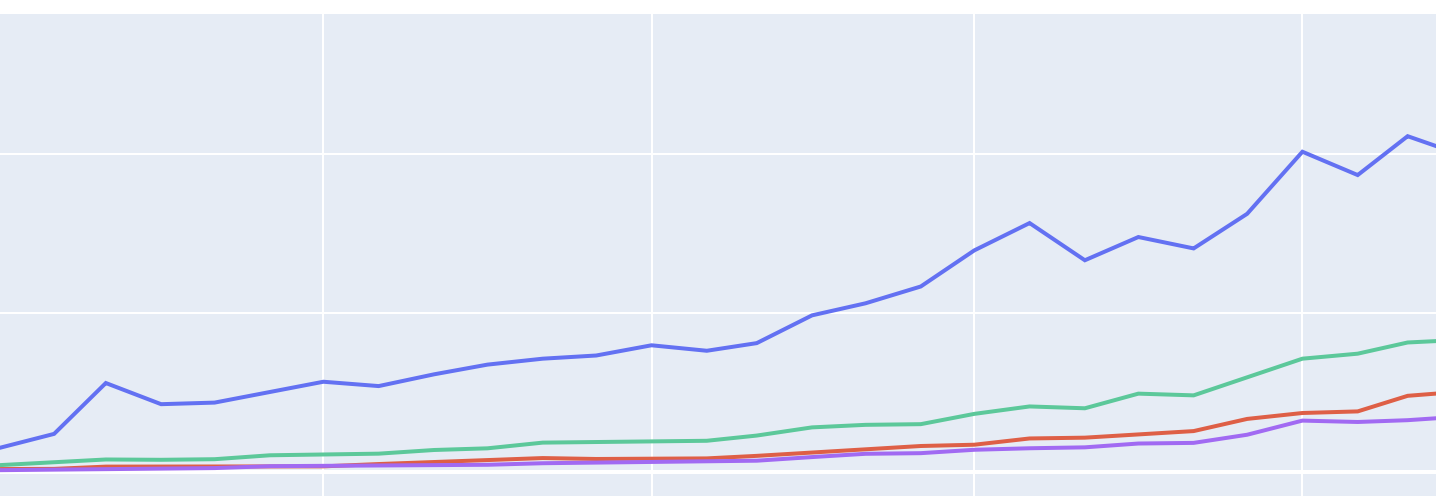
\includegraphics[width=5in]{img/line_chart.png}
  \caption{Line chart}
  \label{fig2.2}
\end{figure}
\\
\pagebreak
\paragraph{Line chart(Figure 2.1)}
We use them when we want to move the focus on the evolution of our data in time, especially when comparing different classes of data.\\
In this example we can see the evolution in time of the number of active editors of different language communities. In the next chapter we will focus more on this concept.
\\
\begin{figure}[!ht]
  \centering
  \setlocalecaption{english}{figure}{Figure}
  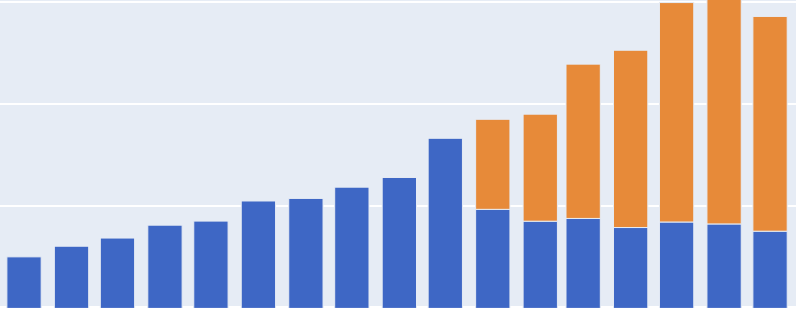
\includegraphics[width=5in]{img/stacked_barchart.png}
  \caption{Stacked bar chart}
  \label{fig2.3}
\end{figure}
\\
\paragraph{Stacked bar chart (Figure 2.2)}
It is particularly suited to analyze the data distribution and focus on the quantity of a certain value with respect to other values. It is the most frequent chart. Different classes of data sharing some common attributes get stacked to render the idea of their quantitative difference.
In this example we see the distribution of two different generations of editors through the years.
\\
\begin{figure}[!ht]
  \centering
  \setlocalecaption{english}{figure}{Figure}
  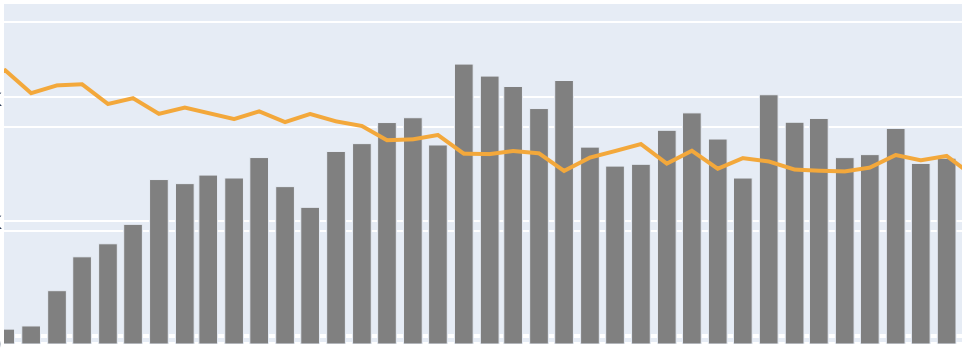
\includegraphics[width=5in]{img/dual_axis_graph.png}
  \caption{Dual-axis graph: line chart and bar chart}
  \label{fig2.4}
\end{figure}
\\
\paragraph{Dual-axis graph (Figure 2.3)}
Helps conveying multiple information at the same time. In fact, in the dashboards it is used in its line chart plus bar chart configuration, thus, it helps the user to analyze the distribution of a certain data class and also compare it to the evolution in time of another class of data. In this example, we can see the distribution of registered editors with respect to the evolution in time of the number of editors that remain active after a certain temporal threshold. Again, this will be explained later.
\pagebreak
\\
\begin{figure}[!h]
  \centering
  \setlocalecaption{english}{figure}{Figure}
  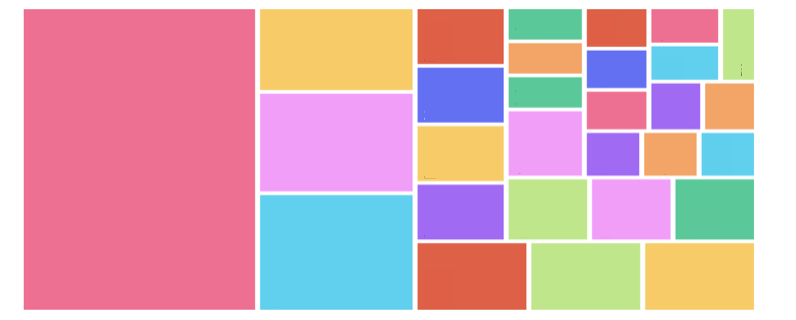
\includegraphics[width=5in]{img/treemap.png}
  \caption{Treemap chart}
  \label{fig2.5}
\end{figure}
\\
\paragraph{Treemap chart (Figure 2.3)}
Finally, the Treemap chart. It is a special graph used to represent the quantitative distribution of certain data classes with respect to all the other data classes considered in the current analysis. \\It is preferred to a pie chart visualization because the comparison between rectangular shapes is clearer than the contrast between circular sectors. Each colorful square can be expanded, to reveal other information about the current object, in this case the current language.\cite{treemap}\\
In the dashboards it is used to visualize the Meta-Wiki participation of the all the Wikipedia language communities.

\section{Dash}
\label{sec:dash}

Dash is the web framework on which the Plotly apps run. It is tailored to create visual dashboards in an extremely simple way. \cite{dash}\\
The entire dashboards layout is built with Dash. There is no HTML, no CSS nor JavaScript.\\
The layout is, however, built with components of the HTML Python module that allows to place HTML classic components, like \verb#div# container or radio buttons, and handling them with a JSON-like syntax. These components directly communicate with the Plotly graphs thanks to the Dash functions, or callbacks, that feed the information coming from them to the Plotly charts, making them interactive. Not only the graphs are interactive, the whole page is: by selecting the desired vital sign, the layout will automatically display the respective dashboard.

\lstset{frame=lines}
\lstset{label={lst:code_direct}}
\lstset{basicstyle=\footnotesize}
\lstset{caption=Structuring the Dash layout}
\begin{lstlisting}
import dash
from dash import Dash, dcc, html, dbc

html.Div(
        html.P('Select Yearly or Monthly Time aggregation'),
        
        html.Br(),
        
        html.Div(
            dcc.Dropdown(
                id='language',
                multi=True,
                value='English (en)',
                style={'width':'490px'}
            ), style={'display':'inline-block','width':'500px'}
        )
    )
    
\end{lstlisting}

From the code snippet above, we can clearly see the absence of any HTML code.
The whole layout is implemented using Python scripts like this.\\
Dash has many libraries as well, such as dash core components (\verb#dcc#) and dash bootstrap components (\verb#dbc#), that provides HTML components with pre-built CSS style, in order to help us build an homogeneous and  elegant web page. Since we want to focus on the dashboards, the layout is designed to be minimal.\\
From the example above, in fact, we can see a drop down in a HTML \verb#Div#. This element comes from the \verb#dbc# library and provides a simple custom drop down menu:
\begin{itemize}
    \item \textbf{id}: since it is an HTML element, we can set its identifier
    \item \textbf{multi}: we can set if it must contains more than one choice
    \item \textbf{value}: it allows us to set the default value, in this case the English language
    \item \textbf{style}: we can add other information about the CSS style
\end{itemize}

All these graphic components hide more than what we see: they are the interface through which we can interact with the Plotly charts.
We can bind these components with functions, called Dash callbacks, that communicate directly with the Graph objects.\\
We also said that Dash is responsible for the whole business logic of the web applications. Let us take a look at the callbacks and how they are defined.

\lstset{frame=lines}
\lstset{label={lst:code_direct}}
\lstset{basicstyle=\footnotesize}
\lstset{caption=Dash callback for URL update}
\begin{lstlisting}
import dash
from urllib.parse import urlparse, parse_qsl, urlencode

@app.callback(Output('page-content', 'children'),
              inputs=[Input('url', 'href')])
def page_load(href):
    if not href:
        return []
    state = parse_state(href)
    return layout1
    
\end{lstlisting}

From the code snippet above we see the definition of a Dash callback.
It works just like a function: we define the input and the output structure, and we write the code to execute. The main thing to notice is that we bind this function to the Dash application with the \verb#@app.callback# string.\\
In this example we are looking at the function that allows the sharing of the visualization with other users: the parameters that are read from the graph callbacks are embedded in the URL, in order to let the page update its HTML components' value with the values read from the URL. In this way, the callbacks will always read the correct parameters. We will read the default ones only if we are visiting the dashboard as a new visitor.\\
In the next chapter, we will have a closer look at this mechanism.\\


\section{Pandas}
\label{sec:pandas}

Pandas is the mediator between front-end and back-end code. \cite{pandas} \\
It is a Python module that is in touch both with Plotly and with the SQL database, managing the data flow between these two components.\\
It is mainly used to encapsulate the result sets coming from the SQL queries asked to the Eurecat Database. Since this data is still too raw, we need to process them in a way that they can work properly with Plotly: we use Pandas objects called Data frames. \\
The Pandas data frames are extremely useful, since they allow us to grab the raw data and envelope them into objects that are much more malleable than their raw form: they have a lot of methods to handle themselves. Let us take a look at how data frames are created:\\

\lstset{frame=lines}
\lstset{label={lst:code_direct}}
\lstset{basicstyle=\footnotesize}
\lstset{caption=Creating a Pandas data frame}
\begin{lstlisting}
import pandas as pd
import sqlite3

conn = sqlite3.connect(database)

SQL_query = '''select * 
            from vital_signs_metrics 
            where topic = 'active_editors' 
                and year_year_month = '''+time_type+'''
                and m1_calculation = 'threshold' 
                and m1_value = '''+user_type+'''  
                and langcode IN (%s) '''%languages

df = pd.read_sql_query(SQL_query, conn)
print(df[:100])
df['percentage']=((df['m2_count']/df['m1_count'])*100).round(2)
    
\end{lstlisting}

First of all, we specify the database with the Sqlite3 connection object \verb#conn#. Then, we create a parameterized SQL query.\\
The parameters of this query are:
\begin{itemize}
    \item \textbf{time type}: it specifies the time aggregation of the final chart, that can be yearly or monthly.
    \item \textbf{user type}: it specifies if we talk about active editors or very active editors.
    \item \textbf{languages}: it determines the desired languages on which we want to do our research.
\end{itemize}
The query is then passed to the database and, at the same time, the result set is put into the data frame \verb#df#. We then print it to ensure that it is the correct desired data set.\\
Finally, we create a new data frame column from already existing ones. In the example above, we create a percentage column.\\ 
If we wanted to do this via SQL, we would have to change the query and thus, we would have put two different things at the same time, violating the Separation of Concern principle \cite{soc}.\\ Instead, with this method we can launch a high level query and then refining it with Pandas. This is much more convenient since we can separate the creation of the raw result set and then the refining phase, making it easier to eventually debug.\\
Later on we will have an in-depth view on how Pandas and Plotly work together.

\section{Architecture}
\label{sec:architecture}
Now that the Python module have been described, this section illustrates how they are structured.

\begin{figure}[!ht]
  \centering
  \setlocalecaption{english}{figure}{Figure}
  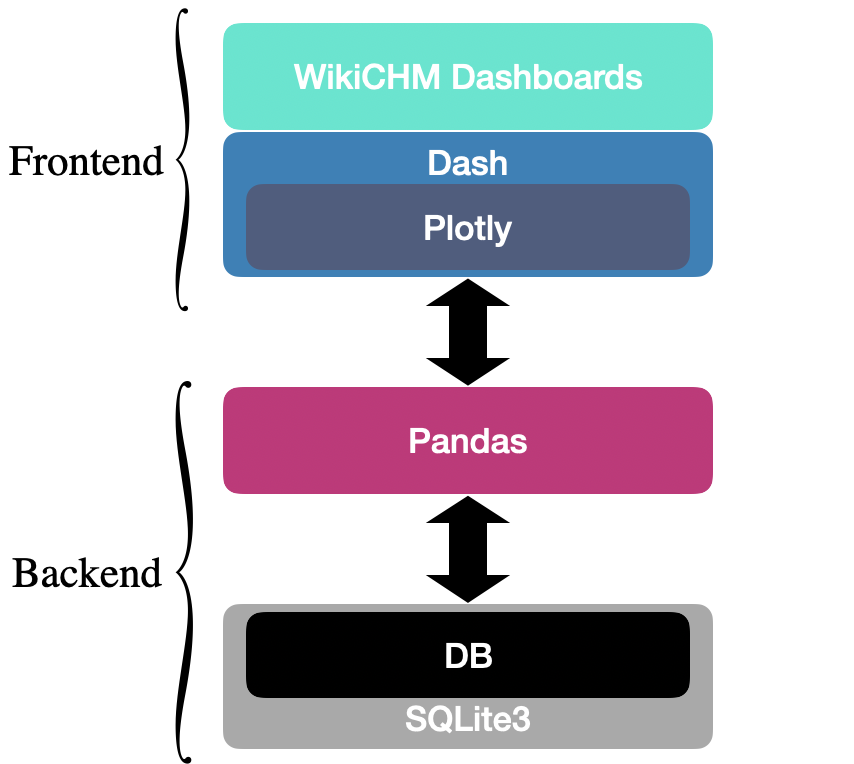
\includegraphics[width=3in]{img/architecture.png}
  \caption{Dashboards architecture}
  \label{fig:arch}
\end{figure}

The Figure \ref{fig:arch} is a high-level definition of the architecture of the visual dashboards. \\
Every level of this structure has been made with ad-hoc Python modules.\\
Let us describe them with a top-down approach:
\begin{itemize}
    \item \textbf{Plotly}: every dashboard's graph is made with the Python library for data visualization. It is contained into Dash web framework to allow the interaction between the user and the HTML components.
    It is what the user actually sees and interacts with
    
    \item \textbf{Dash}: the charts run in a web container, realized with a Python module that allows the creation of web applications. Dash automatically manages every web-related aspects such as the building of the entire layout that can totally change at run-time, creating the website to which the user can access to. \\
    Dash is also responsible for the functions that make the dashboard interactive and for the dynamic layout
    
    \item \textbf{Pandas}: the data plotted are handled with the widely-used data manipulation Python library, handling and managing the exchange of data between the underlying DBMS and the above layers. It is the mediator between the front-end dashboards and the back-end data.
    
    \item \textbf{SQLite3}: this low-level module provides the connection with the relational database, created by the Eurecat researchers, and mainly acts as its DBMS. It is the responsible for raw extraction of the data.
\end{itemize}
Every layer of the structure dialogues with its neighbour.
The data flow bottom up: from the database to the Wiki Community Health Metrics dashboards.\\
Each component captures the output of the underlying layer, elaborates it, and feed its own result to the overlying one.
All these Python modules have been chosen for their mutual compatibility, in particular Python, Dash and Pandas to ensure a smooth and robust workflow.

\space